%%%%%%%%%%%%%%%%%%
% Standalone document
\documentclass[notes.tex]{subfiles}
\begin{document}
%%%%%%%%%%%%%%%%%%%%%%%%%%%%%%%%%%%%%%%%%%%%%%%%%%%%%%%
%%%%%%%%%%%%%%%%%%%%%%%%%%%%%%%%%%%%%%%%%%%%%%%%%%%%%%%
\chapter{Sparticle phenomenology}
\label{chap:pheno}
%%%%%%%%%%%%%%%%%%%%%%%%%%%%%%%%%%%%%%%%%%%%%%%%%%%%%%%
%%%%%%%%%%%%%%%%%%%%%%%%%%%%%%%%%%%%%%%%%%%%%%%%%%%%%%%
In this chapter we discuss the phenomenology of supersymmetric models and how to search for low-energy particle realisations of supersymmetry in experiments. We begin by returning to supersymmetry breaking in order to define some reasonable and (partially) motivated subsets of the 124 MSSM parameters which can be used to define more constrained models. We then discuss supersymmetry at lepton and hadron colliders, and finally look at precision measurements that are indirectly sensitive to the existence of sparticles.


%%%%%%%%%%%%%%%%%%%%%%%
\section{Models for supersymmetry breaking} 
%%%%%%%%%%%%%%%%%%%%%%%
Let us begin by taking a closer look at the models we use to motivate supersymmetry breaking, and what their phenomenological consequences are. This is important to keep in mind as most searches for supersymmetry are interpreted under certain assumptions on the supersymmetry  breaking mechanism.

Generically such models can be illustrated as shown in Fig.~\ref{SSB}. There is one or more {\bf hidden sector} (HS) scalar superfield $X$ -- by hidden we mean that it has no or very small direct couplings to the MSSM fields -- that has an {\it effective (non-renormalizable) coupling} to the MSSM scalar fields $\Phi_i$ of the form
\begin{equation}
\mathcal{L}_\text{HS} = -\frac{1}{M}(\bar\theta\bar\theta)X\Phi_i\Phi_j\Phi_k,
\label{eq:HS_MSSM}
\end{equation}
where $M$ is some large scale, {\it e.g.}\ the Planck scale, that suppresses the interaction. Figure \ref{SUSYB} shows interactions that can lead to such terms, where $M$ is the mass scale of some {\bf mediator} particle $Y$. 

\begin{figure}[h!]
\centering
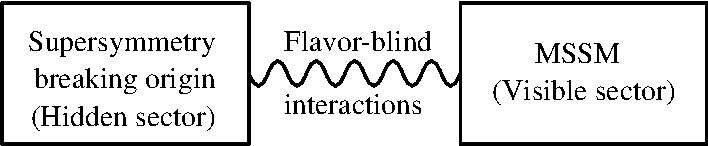
\includegraphics[scale=1.0]{figures/structure} 
\caption{A generic illustration of how to generate soft breaking terms~\cite{Martin:1997ns}. \label{SSB}}
\end{figure}

\begin{figure}[h!]
\begin{center}
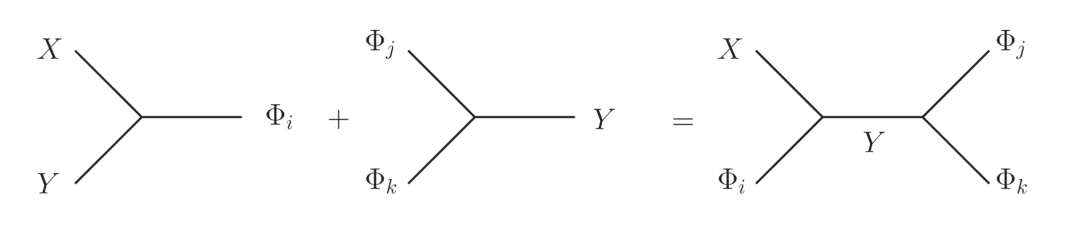
\includegraphics[scale=0.9]{figures/SUSYB} 
\caption{Interactions leading to effective 4-particle couplings in our example. \label{SUSYB}}
\end{center}
\end{figure}

If the hidden sector is constructed so that $X$ develops a vev for its auxillary $F$-component field, $F_X$,\begin{equation}
\langle X \rangle = \theta \theta \langle F_X \rangle,
\end{equation}
it breaks supersymmetry spontaneously, see the discussion leading up to Eq.~(\ref{eq:Fbreaking}). As a result, the interaction in  (\ref{eq:HS_MSSM}) will produce a soft-term of the form of the second term in Eq.~(\ref{eq:soft_terms_component_fields}),
\begin{equation}
\mathcal{L}_\text{soft}=-\frac{\langle F_X \rangle}{M}A_iA_jA_k,
\end{equation}
with the soft-mass parameter
\[m_\text{soft} = \frac{\langle F_X \rangle}{M}.\]
This has reasonable limits in that $m_\text{soft}  \to 0$ as $\langle F_X \rangle \to 0$, which is the limit of no supersymmetry breaking, and $m_{\rm soft} \to 0$ as $M \to \infty$, where the interaction with the hidden sector is decoupled because the mediating particle $Y$ becomes too heavy to have any influence. 

We will now look at two possible ways to construct such a hidden sector called Planck-scale Mediated Supersymmetry Breaking (PMSB) and Gauge Mediated Supersymmetry Breaking (GMSB).


%%%
\subsection{Planck-scale Mediated Supersymmetry Breaking (PMSB)}
%%%
In Planck-scale mediated supersymmetry breaking (PMSB) we blame some gravity mechanism for mediating the supersymmetry breaking from the hidden sector to the MSSM so that the scale of the breaking is $M = M_P = 2.4 \cdot 10^{18}$\,GeV. Then we need to have $\sqrt{\langle F_X\rangle} \sim 10^{10}-10^{11}$\,GeV in order to get $m_{\rm soft} \simeq 50-5000$\,GeV, which is roughly of the right magnitude not to re-introduce the hierarchy problem. The use of $\sqrt{\langle F_X\rangle}$ is just a conventional shorthand notation for the magnitude of the vev of whichever $F$-term that breaks supersymmetry. This is called the {\bf supersymmetry breaking scale}.

The complete soft terms for such a mechanism can then be shown to be
\begin{eqnarray}
\mathcal{L}_\text{soft} &=& -\frac{\langle F_X \rangle}{M_P}\left(\frac{1}{2} f_i \lambda^a_i \lambda^a_i + \frac{1}{6} y'_{ijk}A_i A_j A_k + \frac{1}{2}\mu'_{ij}A_iA_j + \frac{\langle F_X \rangle^*}{M_P^2}x_{ijk}A_i^*A_jA_k + {\rm c.c.}\right)\nonumber\\
 &&- \frac{|\langle F_X \rangle |^2}{M_P^2}k_{ij}A_iA_j^*.
 \end{eqnarray}
Incidentally, we can now see why we assumed the maybe-soft breaking terms to be unimportant, as  in this model they are suppressed by $|\langle F_X \rangle|/M_P^2$ compared to the other masses. 

If one assumes a minimal form for the parameters at the GUT scale, motivated by the wish for unification, {\it e.g.}\ $f=f_i$, $y'_{ijk} = \alpha y_{ijk}$, $\mu'_{ij} = \beta \mu$, and $k_{ij} = k\delta_{ij}$, then all the soft terms are fixed by just four parameters
\[m_{1/2} = f\frac{\langle F_X \rangle}{M_P}, \indent m_0^2 = k \frac{|\langle F_X \rangle|^2}{M_P^2}, \indent A_0 = \alpha \frac{\langle F_X \rangle }{M_P}, \indent B_0 = \beta\frac{\langle F_X \rangle}{M_P}.\]
The resulting phenomenology is called {\bf minimal supergravity}, or {\bf mSUGRA/CMSSM}. This is minimal in the sense of the form of the parameters, and is the most studied, but perhaps not best motivated, version of the MSSM. Usually, $B_0$ and $|\mu|$ are exchanged for $\tan\beta$ at low scales using the EWSB condition  in Eq.~(\ref{eq:EWSB_condition}), so it is common to say that there are four and a half parameters in the model: $m_{1/2}$, $m_0$, $A_0$, $\tan\beta$ and ${\rm sgn}\,\mu$.


%%%
\subsection{Gauge Mediated Supersymmetry Breaking (GMSB)} 
%%%
An alternative to PMSB is gauge-mediated supersymmetry breaking where soft terms come from {\it loop diagrams} with {\bf messenger} superfields that get their own mass by coupling to the hidden sector supersymmetry breaking  vev, and that have Standard Model gauge interactions. By dimensional analysis we must have
\[m_{\rm soft} = \frac{\alpha_i}{4\pi}\frac{\langle F \rangle}{M}.\]
If now the supersymmetry breaking scale  $\sqrt{\langle F\rangle}$ and the messenger mass $M$ are roughly comparable in size, which is reasonable given where the messenger mass comes from, then $\sqrt{\langle F \rangle} \simeq 100$\,TeV can give a viable sparticle spectrum. Notice that there is now a lot less RGE running for the parameters in the GMSB compared to the PMSB since the soft masses are created at a rather low scale.

One way of thinking about how these mass terms appear is that the messenger field(s) get masses from hidden sector vevs and contribute to for example gaugino mass terms through diagrams such as the one in Fig.~\ref{fig:GMSB}, where messenger scalars and fermions run in the loop, and their masses from the hidden sector vevs are symbolised by the mass insertions. Note that scalars can only get mass contributions like this at two-loop order since the messenger interaction is a gauge interaction, involving gauge bosons or gauginos in the MSSM. In order not to spoil GUT unification messengers are often assumed to have small mass splittings and come in $N_5$ complete $\mathbf{5} + \overline{\mathbf{5}}$ (fundamental) representations of $SU(5)$.

\begin{figure}[h!]
\begin{center}
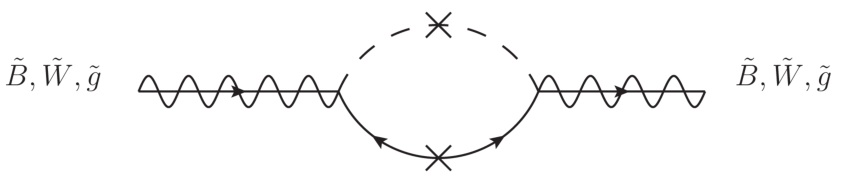
\includegraphics[scale=0.8]{figures/GMSB} 
\caption{Diagram for GMSB giving masses to the gauginos. The messenger scalars and fermions run in the loop.\label{fig:GMSB}}
\end{center}
\end{figure}

The minimal parametrisation of GMSB models is in terms of the scale $\Lambda = \frac{\langle F\rangle}{M}$, the messenger mass $M$, the number of representations $N_5$, and $\tan\beta$ for the EWSB criterion (instead of $\mu$ and $b$). This gives the soft masses
\begin{eqnarray}
M_i &=& \frac{\alpha_i}{4\pi}\Lambda N_5,\quad\text{(gaugino masses)}\label{eq:GMSBgauginomass}\\
m_j^2 &=& 2\Lambda^2 N_5 \sum C(R)_i\left(\frac{\alpha_i}{4\pi}\right)^2,\quad\text{(scalar masses)}
\end{eqnarray}
where the sum is over the quadratic Casimir invariant for the scalar superfield $\Phi_j$ that the scalar field belongs to. We clearly see that the scalar soft-masses are a two-loop effect as discussed above. 

While this parameterisation looks independent of $M$, the messenger scale sets the starting point of the RGE running of the sparticle masses, and thus influences their magnitude. For example, the tri-linear soft-term couplings $a_{ijk}$ are expected to be very small at the messenger scale, and are effectively set to zero, however, due to RGE running they are small, but non-zero at the electroweak scale. Since the scalar masses $m_j$ scale as $\sqrt{N_5}$ compared to $N_5$ for the gauginos, we in general expect the scalars to be lighter in GMSB models. One should also notice that this parameterisation  gives the same hierarchy of gaugino masses as in mSUGRA, $M_3>M_2>M_1$, since (\ref{eq:GMSBgauginomass}) is ordered in terms of the strength of the gauge couplings $\alpha_i$. The origin of the hierarchy is different since in mSUGRA it comes from the running of the parameters down from the GUT scale.



%%%%%%%%%%%%%%%%%%%%%%
\section{Supersymmetry at lepton colliders}
%%%%%%%%%%%%%%%%%%%%%%
Most lepton colliders are $e^+e^-$-colliders, although plans are being made for a muon collider where there is less bremsstrahlung because of the higher muon mass, meaning that higher energies can be reached. The highest energy so-far at an $e^+e^-$-collider was 209 GeV CoM-energy at LEP2 in 2000.

Most supersymmetry searches at lepton colliders rely on pair production from $e^+e^-\to \gamma^*/Z^*$ to set limits, and for R-parity conserving supersymmetry we (again) rely on misisng energy $\slashed{E}$ as an essential signature, however, since the longitudinal momentum is now exactly known full energy conservation can in principle be used. In practice this is challenging at high energies because of collinear Bremsstrahlung. This will be a particularly difficult for a future $0.5-3.0$ TeV CoM International Linear Collider (ILC) or the Compact LInear Collider (CLIC) project.\footnote{For more information on these projects see the websites for the International Linear Collider \url{http://www.linearcollider.org/} and the Compact LInear Collider \url{http://clic-study.org/}}

We can estimate the amplitude of the sfermion pair production process shown in Fig.~\ref{LCPP}. We can write down the matrix element as:
\begin{equation}
\mathcal{M} = \overline{v}ie\gamma^\mu u \frac{-ig_\mu{}_\nu}{k^2+i\epsilon}[-ie\cdot e_f (p_1-p_2)^\nu],
\end{equation}
which gives a squared matrix element of, assuming that the CoM  $s$ is much greater than $m_Z$ and taking into account both the photon and the $Z$:
\begin{equation}
|\mathcal{M}|^2 \simeq \frac{g^4 e_f^2}{8\cos\theta_W}\frac{st+(m_{\tilde{f}}^2-t)^2}{s^2}\times (1+(4\sin^2\theta_W-1)^2).
\end{equation}
We take safely take $(1+(4\sin^2\theta_W-1)^2)\simeq1$. The complete differential cross-section is then:
\begin{equation}
\frac{d\sigma}{dt} = \frac{1}{32\pi}\frac{1}{s^2}|\mathcal{M}|^2.
\label{eq:sfermion_production_diff_xsec}
\end{equation}
This cross section is small due to the coupling factor $g^4$ and sfermion mass suppression. 
\begin{figure}[h!]
\begin{center}
\includegraphics[width=0.5\textwidth]{figures/LCpp.eps} 
\caption{Feynman diagram for the pair production of left-handed sfermions in the s-channel at a linear collider.\label{LCPP}}
\end{center}
\end{figure}

For charginos and neutralinos, as in the case of hadron colliders, the production cross section depends on their wino, bino and higgsino components. The selectron and electron sneutrino have a special r\^ole for $e^+e^-$ colliders due to t-channel diagrams. Figure \ref{fig:tdiag} shows the t-channel diagrams that are important in pair production at a $e^+e^-$ collider.  We show an example of the slepton pair production cross section including the $Z$-resonance at low energies and the t-channel contributions from neutralinos in Fig.~\ref{fig:slepton_xsec}.
Neutralino pair production with t-channel selectron exchange does not suffer from the same problems as neutralino pair production at a hadron collider in the s-channel. However, the process depends on the selectron mass as $m_{\tilde e}^{-4}$ for large mass values.

\begin{figure}[h!]
\begin{center}
\includegraphics[width=\textwidth]{figures/tdiaglc.eps} 
\caption{The t-channel diagrams for pair production of selectrons and electron sneutrinos a) and gauginos b).\label{fig:tdiag}}
\end{center}
\end{figure}

\begin{figure}[h!]
\begin{center}
\includegraphics[width=0.9\textwidth]{figures/sleptons.eps} 
\caption{Cross sections for selectron pair production as a function of energy. The cross sections for ${\tilde e}_L^*{\tilde e}_L$ (solid line), ${\tilde e}_R^*{\tilde e}_R$ (dashed line), and ${\tilde e}_L^*{\tilde e}_R$ (dashed dotted line) are shown separately. The particular model point has a common slepton mass of $m_{\tilde e_{L/R}}=35$ GeV. \label{fig:slepton_xsec}}
\end{center}
\end{figure}

Should a signal be found the parameters of the new particles can be {\it precisely measured} at a lepton collider. either through threshold scans of cross section where the cross section is measured as a function of $\sqrt{s}$. Or, through kinematical distributions, {\it e.g.}\ in $e^+e^-\to \tilde{l}^+\tilde{l}^- \to l^+l^- \tilde{\chi}^0_1\tilde{\chi}^0_1$ the energy distribution for the final state leptons is a uniform distribution between $E_{\rm min}$ and $E_{\rm max}$ where
\begin{equation}
E_{\rm max/min} =\frac{\sqrt{s}}{4}\left(1-\frac{m^2_{\tilde{\chi}^0_1}}{m_{\tilde{l}}^2}\right)\left(1\pm \left(1-\frac{4m_{\tilde{l}}^2}{s}\right)^{1/2}\right).
\end{equation}


%%%
\subsection{Current bounds at lepton colliders}
%%%
The below bounds are all from the LEP (Large Electron Positron) collider, running from 1989 until 2000, which outdated all previous bounds with a top energy of $\sqrt{s}=209$ GeV, recording an integrated luminosity of 233~pb$^{-1}$ above 204 GeV. Results exist from all four LEP experiments ALEPH, DELPHI, L3 and OPAL.\footnote{Most of which are silly acronyms of course.} The numbers are all taken from the PDG (Particle Data Group) review~\cite{Agashe:2014kda}. While these bounds often come from pair-production of the relevant sparticles, and thus are less modell dependent than the hadron collider bounds, there remains some model dependence in many results, which, unfortunately, is sometimes ignored in the litterature. Complicating matters is a reliance by the LEP experiments on theoretical assumptions such as GUT-scale coupling and gaugino mass unification.
\begin{itemize}
\item Selectron: $m_{\tilde{e}_L}>107$ GeV and $m_{\tilde{e}_R}>73$ GeV (ALEPH 2002) in searches for acoplanar di-electrons.\footnote{The observant reader will notice that two electrons are always in the same plane, however, when experimentalists say acoplanar, they mean not in one plane with the beam axis.} The limit is the result of a scan over MSSM parameter space assuming a common $m_0$ and $m_{1/2}$ at GUT scale. Interpreted in mSUGRA with $A_0=0$ the bounds are 152 GeV and 95 GeV, respectively. Due to strict limits on the measured $Z$-width, there is a model independent limit of $m_{\tilde{e}_{L/R}}>40$ GeV.\footnote{Similar model independent limits around half the $Z$-mass exists for all sparticles that couple to the $Z$.}
\item Smuon: $m_{\tilde{\mu}_R}>94$ GeV (DELPHI 2003). The limit is obtained as in the MSSM scenario for the selectron.
\item Stau: $m_{\tilde{\tau}_1}>81.9$ GeV (DELPHI 2003) assuming exclusive $\tilde{\tau}_1 \to \tau \tilde{\chi}^0_1$ and $m_{\tilde{\tau}_1} - m_{\tilde{\chi}^0_1}> 15$ GeV.
\item Sneutrinos: From the Z-width we can obtain the model independent limit $m_{\tilde{\nu}}> 44.7$ GeV. From collider experiments we have $m_{\tilde{\nu}}>94$ GeV (DELPHI 2003) in neutralino \& slepton searches. This assumes $m_{\tilde{e}_R} - m_{\tilde{\chi}^0_1}>10$ GeV.
\item Neutralino: $m_{\tilde{\chi}^0_1}> 46$ GeV (DELPHI 2003). This limit is derived from the direct searches for $\tilde{\chi}^\pm_1 \tilde{\chi}^0_2$ and $\tilde{\chi}^0_1 \tilde{\chi}^0_2$. This assumes gauge coupling unification and a common gaugino mass $m_{1/2}$ at GUT scale. Even in the Z-decays, the contribution depends on the higgsino part in the lightest neutralino, so $m_{\tilde{\chi}^0_1} \simeq 0$ GeV is in principle allowed~\cite{Dreiner:2009ic}.
\item From the $Z$-width we can extract a strict limit of $m_{\tilde{\chi}^\pm_1}\geq 45$ GeV.
We also have $m_{\tilde{\chi}^\pm_1}\geq 94$ GeV (DELPHI 2003), assuming GUT scale universality of $m_0$ and $m_{1/2}$ and using multiple direct search channels from production of charginos, neutralinos and sleptons. It also assumes either no third generation mixing or $m_{\tilde{\chi}^\pm_1} - m_{\tilde{\chi}^0_1}>6$ GeV. 
\end{itemize}




%%%%%%%%%%%%%%%%%%%%%%
\section{Supersymmetry at hadron colliders}
%%%%%%%%%%%%%%%%%%%%%%
Let us first point out some more or less obvious points.\footnote{You might find these very obvious, they are, however, quite important and some theory people seem oblivious to them.}
\begin{enumerate}[1)]
\item Hadron colliders collide quarks and gluons. This means that we get large cross sections only for QCD charged sparticles, {\it i.e.}\ squarks and gluinos, provided their masses are low enough. 
\item  As discussed earlier, with R-parity conservation (RPC) sparticles are produced in pairs and both decay to the LSP.
\item Illustrated in Fig.~\ref{cascade1} these sparticles can decay to the LSP in many different, and potentially complicated, cascades. The possible decays for a particular MSSM model point called SPS1a is shown in Fig.~\ref{cascade2}. We should realize that many of these decays are hard to distinguish from ordinary SM (background) processes, or just undetectable.
\item Standard Model backgrounds have much, much bigger cross sections. Figure~\ref{LHCbackground} shows the expected backgrounds and signals produced in different channels at the 14 TeV LHC for different particle masses.
%\begin{figure}[h!]
%\centering
%\includegraphics[scale=0.5]{figures/detector.eps} 
%\caption{How detectors work.\label{detector}}
%\end{figure}
\item R-parity conservation gives you {\bf missing transverse energy} $\slashed{E}_T$ at hadron colliders due to the escaping LSPs, {\it i.e.}\ an imbalance in the directional sum of all energy deposits transverse to the beam direction. There is no logitudinal energy balance in a hadron colllider because the energies of the colliding partons are not known.
\end{enumerate}

\begin{figure}[h!]
\centering
\includegraphics[width=0.95\textwidth]{figures/cascade1.eps} 
\caption{Diagram of a possible collision process in the LHC for an RPC model. Illustration by C.\, Lester~\cite{Lester:TOOLS2012}.\label{cascade1}}
\end{figure}

\begin{figure}[h!]
\centering
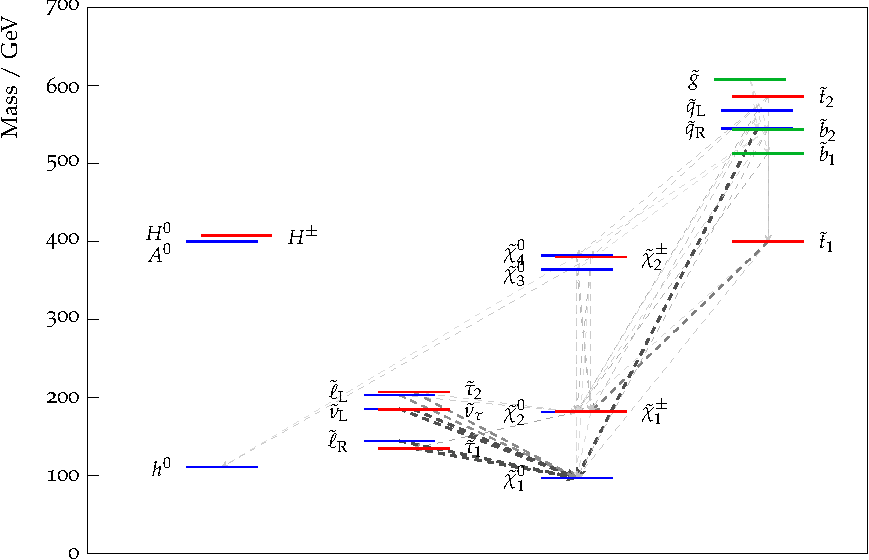
\includegraphics[width=0.95\textwidth]{figures/sps1a.eps} 
\caption[Cascades for SPS1a]{Possible sparticle cascades for the SPS1a model point. Only decays with branching rations above 5\% are shown. The line width indicates relative branching ratios. The plot was generated using {\tt PySLHA~3.0.1}~\cite{Buckley:2013jua}. \label{cascade2}}
\end{figure}

\begin{figure}[h!]
\centering
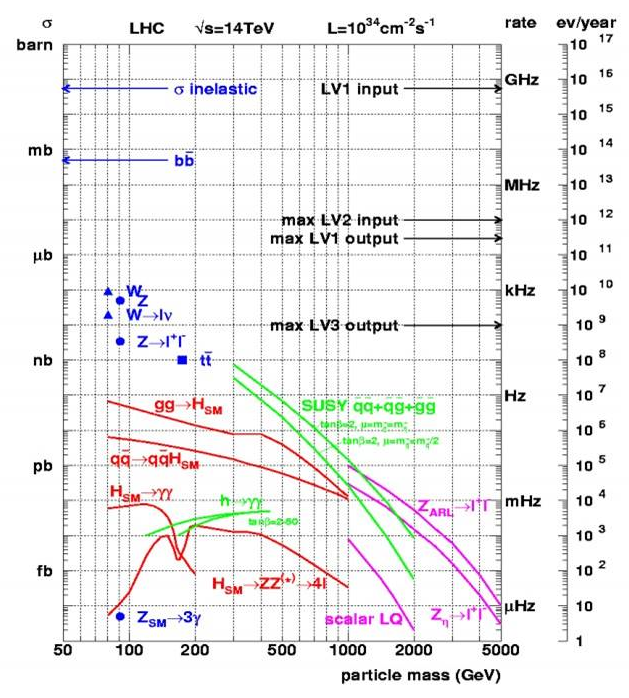
\includegraphics[width=0.7\textwidth]{figures/background.eps} 
\caption{Plot of the expected signals for various processes at the 14 TeV LHC plotted against the mass of the particles. The current Run II of the LHC has collected around 4~fb$^{-1}$ of data, so the fb scale indicates processes where $\mathcal{O}(1)$ events are expected. \label{LHCbackground}}
\end{figure}

The consequences of the above is that we search for events with jet activity---squarks/gluinos decaying to the LSP---and missing energy from two LSPs. One simple way to do this is to define the {\bf effective mass}
\begin{equation}
M_{\rm eff} = \sum p_T^{\text{jet}} + \slashed{E}_T,
\label{eq:Meff}
\end{equation}
and search for deviations from SM expectations. Figure \ref{effectivemassplot} shows a simulation of such a supersymmetry signal at the LHC for a benchmark MSSM model called LHC Point 2. However, there are models where this is ineffective. Imagine a scenario where only the lightest stop $\tilde{t}_1$ is copiously produced. If $m_{\tilde{t}_1} - m_{\tilde{\chi}^0_1}< m_W$ then $\tilde{t}_1 \to c\tilde{\chi}^0_1$ or $\tilde{t}_1 \to b l \nu \tilde{\chi}^0_1$ decays dominate, where all final state particles have low energy ($p_T$), so-called {\bf soft particles}. This is very difficult to discover with standard techniques.
\begin{figure}[h]
\centering
\includegraphics[scale=0.5]{figures/effmass.eps} 
\caption{Plot of the differential cross section with respect to effective mass, plotted against the effective mass of the final state particles as given in (\ref{eq:Meff}). The colored data points represent different SM processes, and the histogram is the sum of all SM contributions, while the white circles represent a possible supersymmetry scenario. The position of the supersymmetry signal maximum is correlated to the masses of $\tilde{\chi}$ and $\tilde{q}$, but there is large variance. \label{effectivemassplot}}
\end{figure}

One alternative to jets and lots of missing energy is to look for leptons (and some small missing energy) from gaugino pair production and decays. Searching the lepton and missing energy channels is a very effective way to isolate any production of sparticles from SM backgrounds, but for setting bounds it is bad since the only model independent production is {\bf Drell-Yan} production, {\it e.g.}\ $q\overline{q}\to (Z/\gamma)^*\to\tilde{\chi}^0_1\tilde{\chi}^0_2,\tilde{\chi}^{+}_1\tilde{\chi}^{-}_1,\tilde{l}_L^*\tilde{l}_L,\tilde{l}_R^*\tilde{l}_R$, and $q'\overline{q}\to W^*\to\tilde{\chi}^0_2\tilde{\chi}^\pm_1$, which all have low cross sections due to the smaller electroweak coupling and the smaller anti-quark content of the proton. The expected bounds from such searches for the mSUGRA model is compared to other searches in Fig.~\ref{fig:reach}.

\begin{figure}[h!]
\centering
\includegraphics[scale=0.5]{figures/reach.eps} 
\caption{Plot of the projected discovery reach for different values of $m_{1/2}$ and $m_0$ in the mSUGRA model with 100~fb$^{-1}$ or 300~fb$^{-1}$ of data at the Compact Muon Spectrometer (CMS). The light blue area represents theoretical restrictions on the parameter space. The dark blue area is the parameter space that was probed by the Tevatron. The red lines represents a pure jets pluss $\not\! E_T$ search at 14\,TeV. The blue lines represent searches using leptons. The dotted lines show the masses of different sparticles in this parameter space. \label{fig:reach}}
\end{figure}

You may ask, why not look for the production of $\tilde{\chi}^0_1\tilde{\chi}^0_1$? To first order the answer might be that with nothing else in the event, we cannot measure the missing energy as that requires an {\it imbalance} in momentum. However, given sufficient QCD radiation from the initial quark/gluon\footnote{For an $e^+e^-$ collider this would be photon radiation from the initial electron/positron.} a single jet recoiling against missing energy could potentially be measured, and this, so-called {\bf mono-jet search}, is indeed a search channel for dark matter production at the LHC. However, for neutralino dark matter this does not work all that well for other reasons. The $Z\tilde\chi_i^0\tilde\chi_j^0$ vertex shown in Fig.~\ref{fig:ZNN}  has the Feynman rule 
\begin{equation}
\frac{ig}{2\cos\theta_W}\gamma^\mu\left[\left(N_{i3}N^*_{j3}-N_{i4}N^*_{j4}\right)P_L-\left(N^*_{i3}N_{j3}-N^*_{i4}N_{j4}\right)P_R\right],
\end{equation}
which depends only on the higgsino components of the neutralinos, $N_{i3}$ and $N_{i4}$. This can be understood from the fact that there are no $ZZZ$ or $Z\gamma\gamma$ vertices in the SM that can be supersymmetrized, only a $Zhh$ vertex. For the photon there is no tree level coupling to the neutralinos at all since there are no direct couplings between the higgs and the photon in the SM. Thus, only neutralinos with significant higgsino components can be produced this way. To top it off, a light higgsino with a mass dominated by the $\mu$ parameter would have very similar values of $N_{i3}$ and $N_{i4}$, thus canceling the coupling.

\begin{figure}[h!]
\begin{center}
\includegraphics{figures/Zgaugino.eps} 
\caption{Coupling $Z\tilde\chi_i^0\tilde\chi_j^0$.\label{fig:ZNN}}
\end{center}
\end{figure}

Should some excess be discovered in any search, we need some smoking duck in order to confirm that this is indeed supersymmetry.  We would like to identify and measure the masses of as many new particles as possible, and hopefully also their spin. To do this, a multitude of techniques have been invented, all facing the problem of how to deal with the loss of information from the LSP. Figure \ref{measurement} shows an example of one such technique where sequential two-body decays of sparticles are used. For the generic decay chain shown in Fig.~\ref{fig:gen_casc} with three sequential two-body decays we can measure the invariant mass between two detectable end-products, $a$ and $b$, $m_{ab}$. Even if the particle $A$ at the end of the chain is invisible one can show that the invariant mass distribution for $m_{ab}$ has a triangular shape with a sharp endpoint at the maximum
\begin{equation}
(m_{ab}^{\max})^{2} = \frac{\left(m_{C}^{2}-m_{B}^{2}\right)
\left(m_{B}^{2}-m_{A}^{2}\right)}{m_{B}^{2}}, 
\label{eq:m_ab}
\end{equation}
where we have assumed that $a$ and $b$ are massless.\footnote{A more complicated expression covers the massive case.} A measurement of this endpoint position gives us one realtionship between the three unknown (sparticle) masses. If we have a chain with three sequential two-body decays we can repeat this measurement with three more possible invariant mass combinations, arriving at four equations with four unknown, which can in principle at least be solved for the masses involved.

\begin{figure}[h!]
\centering
\includegraphics[width=0.8\textwidth]{figures/fig-chain.eps} 
\caption{Generic cascade decay $D\to Cc\to  Bb \to Aabc$~\cite{Miller:2005zp}. \label{fig:gen_casc}}
\end{figure}

\begin{figure}[h!]
\centering
\includegraphics[width=0.9\textwidth]{figures/p250_OSOF_mll.eps} 
\caption{Invariant mass distribution of opposite sign same flavour (OSSF) dileptons for the mSUGRA benchmark model point SPS1a~\cite{Gjelsten:2004ki}. \label{measurement}}
\end{figure}

As alternatives to these standard searches we have searches for decaying LSPs when R-parity is violated, or the production of single sparticles.\footnote{Single sparticle production requires rather large RPV couplings for the $LQ\bar D$ or $\bar U \bar D\bar D$ operators, of the order of $\lambda > 10^{-2}$.} There is the possibility of {\bf massive metastable charged particles} (MMCPs), typically in scenarios with a gravitino LSP, where the next-to-lightest supersymmetric particle (NLSP) is charged and long-lived because the decay to the gravitino is via a very weak gravitational coupling. The latter also includes so-called {\bf R-hadrons} if the NLSP has color charge, which means that it will hadronize after production and be a short-lived but very massive meson or baryon. We should also mention the searches for the extra Higgs states predicted in the MSSM.\footnote{But we really don't have time.}


%%%%%%%%%%%%%%%%%%%%%%%
\section{Current bounds on sparticle masses}
%%%%%%%%%%%%%%%%%%%%%%%
With the LHC running and collecting data the details in this section are continuously becoming out-of-date. We will still try to make some general remarks on the current limits. Most of these limits are from Run I of the LHC at 8 TeV with analysis using up to 20 fb$^{-1}$ of data. This is strongest current limits are on the squark and gluino masses simply because of the production cross section. Bounds on EW gauginos and sleptons exist, but these are either model dependent (depend on squark/gluino mass assumptions and cascade decays), or weaker if the rely only on electroweak production. Direct bounds from the LHC experiments ATLAS and CMS now superseed  bounds from other colliders (Tevatron and LEP) in almost all channels.

\subsection{Squarks and gluinos}
In Fig.~\ref{squarkgluinolimit} we show the most recent limits from ATLAS in the jets plus missing energy channel, using all currently available data at the highest energy of 8 TeV. The limit has been interpreted within the mSUGRA model, where the parameters $\tan\beta$ and $A_0$ have been chosen in order to give relatively large Higgs masses for small values of $m_{1/2}$ and $m_0$. The figure also shows the corresponing first and second generation squark masses, the gluino mass and the higgs mass for these parameter values. From ATLAS we then have the following approximate bounds in mSUGRA: $m_{\tilde{q}}>1600$\,GeV and $m_{\tilde{g}}> 1100$\,GeV.

\begin{figure}[h!]
\begin{center}
\includegraphics[width=0.9\textwidth]{figures/fig_05a.eps} 
\caption{Plot of the excluded area in the $m_{1/2}$-$m_0$ plane of the mSUGRA parameter space for $\tan\beta=30$, $A_0=-2m_0$ and $\mu >0$ . The limit is the red line. The green area is theoretically forbidden because it has a charged LSP (the stau) \cite{ATLAS-CONF-2013-047}.\label{squarkgluinolimit}}
\end{center}
\end{figure}

Notice that in the figure the direct squark mass bound is almost equivalent to the mass required for a sufficiently heavy higgs, thus the direct search does not yet constrain the squarks masses significantly  more than the indirect constraint from the higgs mass. 

An important question is how these bounds change as we move away from the mSUGRA assumptions. By pushing the gluino up in mass using $M_3$ the production cross section falls significantly. Limits of at most  $m_{\tilde{q}}>850$\,GeV assuming only squark production were quoted in the summer 2013 conferences, and the limit falls away entirely if $m_{\tilde{\chi}_1^0}>300$\,GeV becuase the decay products of the squark (quarks) have too little energy.\footnote{The technical term for this is {\bf soft} decay products.} Should one squark generation or flavour be significantly lighter than the others this means a further reduction in the production cross section and thus an even weaker bound. It is also fairly clear that removing R-parity, meaning that the LSP decays, also weakens the above conclusions due to the possible absence of significant missing energy. Thus, despite popular optinion, the generic squark mass bounds outside of specific scnearios like mSUGRA, are currently still fairly weak, in particular compared to indirect bounds via the higgs.

The gluino mass bound is somewhat more robust. Pushing up squark masses and assuming only gluino production gives $m_{\tilde{g}}>1200$\,GeV (when also including CMS results), however, the limit again disappears for $m_{\tilde{\chi}_1^0}>480$\,GeV.

\subsection{Sbottom}
The above bounds on the first and second generation squarks do not apply to the third generation as they are generically lighter and can have more complicated decay signatures. In Fig.~\ref{fig:sbottom} we see current best limits from ATLAS on the lightest sbottom taken from~\cite{Aad:2013ija}. Note that this limit assumes 100\% branching ratio for $\tilde b_1\to b \tilde \chi_0^1$. If this branching ratio  is reduced to 60\% the excluded upper limit on the sbottom mass for $m_{\tilde\chi_1^0} < 150$\,GeV is reduced to 520 GeV. Similarly for $m_{\tilde b_1} = 250$\,GeV, the upper limit on $m_{\tilde\chi_1^0}$ is reduced by 30 GeV.

\begin{figure}[h!]
\begin{center}
\includegraphics[scale=0.5]{figures/fig_05.eps} 
\caption{Plot of the excluded area in the ($m_{\tilde{b}_1}$,$m_{\tilde{\chi}_1^0}$) plane. The limit from ATLAS is the red line, while the green and blue colored areas are excluded from different Tevatron experiments~\cite{Aad:2013ija}.\label{fig:sbottom}}
\end{center}
\end{figure}

\subsection{Stop}
For the stop there are many possible competing decay chanels, meaning that any limit set is very model dependent. The two main decay categories for the lightest stop are via the chargino, if available, $\tilde{t}_1\to b \tilde{\chi}^\pm_1$, and directly to the neutralino $\tilde{t}_1\to t\tilde{\chi}^0_1/ Wb \tilde{\chi}^0_1/ c\tilde{\chi}^0_1$, where the dominant decay mode depends on the stop--neutralino mass difference. A summary of (the many) current ATLAS limits for the stop is found in Fig.~\ref{fig:stop}. It is important to notice the surviving possibility of quite light stops in conjunction with a light neutralino or chargino.

\begin{figure}[h!]
\begin{center}
\includegraphics[width=\textwidth]{figures/stop.eps} 
\caption{Plot of the excluded area in the ($m_{\tilde{t}_1}$,$m_{\tilde{\chi}^0_1}$) plane for the two main decay categories. References for the individual analysis given in figure.\label{fig:stop}}
\end{center}
\end{figure}

\subsection{Sleptons}
As mentioned above the mass bounds on sleptons will be very dependent on the assumed production mechanism. The most model independent bounds come from assuming only electroweak pair production as in \cite{ATLAS-CONF-2013-049}, which presents the results of a search for two opposite-sign same-flavour (OSSF) leptons with missing energy. The result for degenerate right- and left-handed smuons and selectrons, assuming 100\% branching ratio in the neutralino, is shown in Fig.~\ref{fig:slepton}. Individual selectron and smuon limits are significantly weaker. Limits from this kind of search in complete models, such as mSUGRA, are typically much weaker than those that come from searches for jets and missing energy, {\it e.g.}\ see Fig.~\ref{fig:reach}.

\begin{figure}[h!]
\begin{center}
\includegraphics[width=\textwidth]{figures/slepton.eps} 
\caption{Plot of the excluded area in the ($m_{\tilde l}$,\,$m_{\tilde{\chi}^0_1}$) plane for mass degenerate right- and left-handed smuons and selectrons~\cite{ATLAS-CONF-2013-049}.\label{fig:slepton}}
\end{center}
\end{figure}

There are currently no constraining searches for direct pair production of staus.

\subsection{Charginos and neutralinos}
As for the sleptons, bounds are dependent on the production process assumed. With chargino pair production, $\tilde\chi_1^+\tilde\chi_1^-$, the search for two OSSF leptons discussed in the previous subsection again applies because the chargino can decay via a slepton or sneutrino~\cite{ATLAS-CONF-2013-049}. We show the results assuming $m_{\tilde l}=m_{\tilde\nu} = (m_{\tilde\chi_1^\pm} +m_{\tilde\chi_1^0})/2$, and again 100\% branching ratio, in Fig.~\ref{fig:chargino}.

\begin{figure}[h!]
\begin{center}
\includegraphics[width=\textwidth]{figures/chargino.eps} 
\caption{Plot of the excluded area in the ($m_{\tilde\chi_1^\pm}$,\,$m_{\tilde{\chi}^0_1}$) plane~\cite{ATLAS-CONF-2013-049}.\label{fig:chargino}}
\end{center}
\end{figure}

We can also search for $\tilde\chi_2^0\tilde\chi_1^\pm$ production with three leptons and missing energy. 
The results from~\cite{ATLAS-CONF-2013-035}, where 100\% branching ratio into vector bosons is assumed, are shown in Fig.~\ref{fig:cha_neu}.

\begin{figure}[h!]
\begin{center}
\includegraphics[width=\textwidth]{figures/cha_neu.eps} 
\caption{Plot of the excluded area in the ($m_{\tilde\chi_1^\pm}$,\,$m_{\tilde{\chi}^0_1}$) plane assuming $m_{\tilde\chi_1^\pm}=m_{\tilde\chi_2^0}$~\cite{ATLAS-CONF-2013-035}.\label{fig:cha_neu}}
\end{center}
\end{figure}



%%%%%%%%%%%%%%%%
\section{Precision observables}
%%%%%%%%%%%%%%%%
A different way to exclude supersymmetric models is their indirect effect on very accurately measured SM processes, so-called precision observables, through loop diagrams with sparticles. We will here discuss four of the most sensitive probes: electroweak precision observables, the value of the anomolous magnetic moment of the muon $(g-2)_\mu$, the flavour changing neutral current (FCNC) process $b\to s\gamma$ and the very rare (and FCNC) process $B_s\to\mu\mu$.

%%%
\subsection{Electroweak precision observables}
%%%
When we talk about electroweak precision observables, we study parameters such as $M_W$ (or $M_Z$), $\Gamma_W$, $\Gamma_Z$, $m_t$ and $\sin\theta_W$, as well as the Higgs mass $m_h$ and the properties of the Higgs such as its couplings to all the other particles (gauge and Yukawa couplings) and its self-coupling. 

Up to last year we studied all of these as {\it functions} of the unknown Higgs mass, looking for devations that could be a sign of supersymmetry. We show a fit to all available electroweak data and direct exclusion bounds in Fig.~\ref{SMprecexcl} by the {\tt Gfitter} collaboration just before the LHC started taking data, a fit pretty much indicating that the most probable SM Higgs mass was 125 GeV. 

\begin{figure}[h!]
\begin{center}
\includegraphics[width=\textwidth]{figures/SMprecexcl.eps} 
\caption{Plot of the total $\Delta \chi^2$ from all precision variable measurements and the direct exclusions bounds for the SM Higgs from LEP and the Tevatron, as a function of the Higgs mass.\label{SMprecexcl}}
\end{center}
\end{figure}

Figure \ref{mSUGRAprec} shows a similar plot for mSUGRA. At that time the absolute minimum of the fit, even taking into account the different number of parameters, gave a better a better fit for mSUGRA, $\min\chi^2_{\rm mSUGRA}<\min\chi^2_{\rm SM}$, but this changed quickly when the Higgs was found because of the position of the two minima.

\begin{figure}[h!]
\begin{center}
\includegraphics[width=\textwidth]{figures/mSUGRApre.eps} 
\caption{Plot of the $\Delta \chi^2$ from all precision variable measurements for mSUGRA as a function of the Higgs mass. The yellow area shows the experimentally excluded area, while the brown shows the theoretically inaccessible area.\label{mSUGRAprec}}
\end{center}
\end{figure}

Now all the parameters of the SM---neutrinos excepted---have been determined to some precission. Thus the SM is a completely constrained system. If we now do a electroweak fit the situation looks like that in Fig.~\ref{fig:EWfit_LHC2012}, where we show the global fit compared to the measured values of the $W$ and top masses. Clearly what we are seeing here is (still?) consistent with the SM.

\begin{figure}[h!]
\begin{center}
\includegraphics[width=\textwidth]{figures/2013_09_19_W_vs_top_logo.eps} 
\caption{Electroweak fit excluding $M_W$ and $m_t$ (blue), compared to their measured values (green)~\cite{Baak:2012kk}.\label{fig:EWfit_LHC2012}}
\end{center}
\end{figure}

%%%
\subsection{$(g-2)_\mu$}
%%%
The anomalous magnetic moment of the muon, $(g-2)_\mu$, has been very precisely measured by the E821 experiment at BNL \cite{Bennett:2006fi} to be:
\[g_\mu = 2.00116592089(63),\]
or, in terms of $a_\mu$ which is the devation from 2, 
\[a_\mu^{(\rm exp)}=11659208.9(6.3)\cdot 10^{-10},\]
where the parenthesis indicates the uncertainty on the last digits. Figure \ref{moudig} a) shows the lowest order $\mu \to \mu \gamma$ diagram. Loop corrections to this diagram give $a_\mu$. In the SM we find the prediction
\[a_\mu^{\rm SM}=11659183.0(5.1)\cdot 10^{-10},\]
giving a difference with respect to the experimental value of
\[\delta_{a_\mu} \equiv a_\mu^{\rm exp}-a_\mu^{\rm SM} = (25.9\pm 8.1)\cdot 10^{-10},\]
a value which is 3.2$\sigma$ away from zero. This is probably the clearest discrepancy that exists today between the SM and measurements.

However, we should be aware that one of the SM contributions, the so called {\bf hadronic vacuum polarization} as shown in Figure~\ref{moudig} b), involves hadronic loops where one has to rely on experimental information on low energy $e^+e^-\to \gamma^* \to {\rm hadrons}$ in order to estimate a contribution of $a_\mu^{\rm HVP}=10.5(2.6)\cdot 10^{-10}$, which is of the same order of magnitude as the discrepancy, and may be prone to errors in the interpretation. 

\begin{figure}[h!]
\begin{center}
\includegraphics{figures/muonprec.eps} 
\caption{Diagrams for muon interaction with an electromagnetic field. Loop corrections to the tree level diagram a) give the value of $a_\mu$. Diagram b) shows hadronic vacuum polarization where the blob contains QCD fields. Diagrams c) and d) show the lowest order MSSM contributions to $a_\mu$.\label{moudig}}
\end{center}
\end{figure}

One-loop corrections to $(g-2)_{\mu}$ in the MSSM are shown in Figure~\ref{moudig} c) and d). These contribute opposite sign terms $a_\mu(\tilde{\chi}^0)$ and $a_\mu(\tilde{\chi}^-)$. A thorough analysis shows that we need $\mu>0$ in order to give a positive contribution that will close the gap between the experimnetal value and the prediction. In order to get a sufficiently large contribution the loop masses must be less than $500-600$\,GeV for $\tan\beta = 40-50$ and $200-300$\,GeV for $\tan\beta \simeq10$.

\subsection{$b \to s\gamma$}
The process $b \to s\gamma$ is a FCNC process which must proceed through loops. Figure~\ref{btosdiags} a) shows the SM process. This is suppressed by the smallness of the CKM entries, and the large masses $m_W$ and $m_t$.

\begin{figure}[h!]
\begin{center}
\includegraphics[width=\textwidth]{figures/btosdiags.eps} 
\caption{Diagrams for the process $b \to s\gamma$. a) shows the SM diagram while b), c) and d) show MSSM contributions.\label{btosdiags}}
\end{center}
\end{figure}

The process has been measured in decays of the type $B\to X_s\gamma$, {\it e.g.}\  in $B\to K\gamma$, and calculated at NNLO to be ${\rm Br}(B\to X_s\gamma)_{\rm SM} = (3.36 \pm 0.23)\cdot 10^{-4}$ for $E_\gamma \geq 1.6$\,GeV~\cite{Misiak:2015xwa,Czakon:2015exa}.\footnote{For the process $b\to d \gamma$ the SM calculation yields  ${\rm BR} (B \to X_d \gamma) = 1.73^{+0.12}_{-0.22} \cdot 10^{-5}$.}

Supersymmetry may contribute, {\it e.g.} with diagrams such as Fig.~\ref{btosdiags} b) where the  $m_{bs}^2\tilde{b}^*\tilde{s}$ mass term that changes a $\tilde b_1$ to a $\tilde s$ is a soft breaking off-diagonal term, often denoted $\delta_{23}$. The main MSSM contributions are expected to come from chargino--stop\footnote{We usually expect a higher generation off-diagonal terms to be larger due to RGE running controlled by Yukawa couplings.} and charged higgs--top loops, as shown in Figs.~\ref{btosdiags} c) and d), respectively. However,  there is little room for effects from superymmetry  since the current experimental world average is ${\rm Br}(B\to X_s\gamma)=(3.55\pm 0.26)\cdot 10^{-4}$ (PDG 2010). This means that either the charged Higgs is heavy enough and the stop-scharm soft mass term small enough, or that there are cancellations between the contributions. 

%%%
\subsection{$B_s \to \mu^+\mu^-$}
%%%
The process  $B_s \to \mu^+\mu^-$ is another FCNC process as either the bottom or the strange quark must change flavour in order to couple to the muons. The SM process is shown in Fig.~\ref{bsmudiags} a), involving an intermediary $Z$-boson. There is additional suppression from a CKM factor in one of the $W$-vertices, in order to change a third generation quark to a second generation quark, or {\it vice versa}. On top of this, it also suffers from what is called {\bf helicity suppression} in the SM. The $Z$-boson is spin-1, while the starting point meson $B_s$ is spin-0 (pseudoscalar), meaning that the spins of the quarks are opposite. At some point in the diagram the helicity (chirality) must ``flip". This introduces an extra suppression proportional to $m_\mu^2/M_{B_s}^2$, making the expected rate extremely small and sensitive to supersymmetry contributions. We get a similarly supressed process for $B_d$ with a $\bar d$-quark instead of the $\bar s$ in the initial state.

\begin{figure}[h!]
\begin{center}
\includegraphics[clip=true,width=0.45\textwidth,trim=0 4.2cm 0 0]{figures/bsmudiag.eps} 
\includegraphics[width=0.45\textwidth]{figures/pmssm2.eps} 
\caption{Diagrams for the process $B_s \to \mu^+\mu^-$. Diagram a) shows one of the leading SM contributions, while b) shows one contribution from the MSSM taken from~\cite{Bobeth:2001sq}. \label{bsmudiags}}
\end{center}
\end{figure}

The predicted SM branching ratios for these processes are~\cite{Bobeth:2013uxa}:
\begin{eqnarray}
{\rm Br}(B_s \to \mu^+\mu^-) &=& (3.65 \pm 0.23)\cdot 10^{-9},\\
{\rm Br}(B_d \to \mu^+\mu^-) &=& (1.06 \pm 0.09)\cdot 10^{-10}.
\end{eqnarray}
First evidence for the $B_s$ decay was shown by the LHCb collaboration in 2012. The final observation required combining Run I data from both LHCb and CMS, and was published in 2014~\cite{CMS:2014xfa}. The current values are:
\begin{eqnarray}
{\rm Br}(B_s \to \mu^+\mu^-) &=&  2.8^{+0.7}_{-0.6}\cdot 10^{-9},\\
{\rm Br}(B_d \to \mu^+\mu^-) &=&  3.9^{+1.6}_{-1.4}\cdot 10^{-10},
\end{eqnarray}
where one should keep in mind that the $B_d$ decay has only evidence at $3.2\sigma$ significance.

In the MSSM there are contributions from process such as shown in Fig.~\ref{bsmudiags} b). These contributions are proportional to $\tan^6\beta$, which makes the decay process highly sensitive to scenarios with large $\tan\beta$. To see this dependence, notice that $\mu$ couples to the mediating heavy higgses $H/A^0$ through the Yukawa term $y^l_{22} L_2 H_d \overline{E}_2$ in the superpotential, and the Yukawa constant in this term, $y^l_{22} = y_\mu$, is connected to the fermion mass through $m_\mu = y_\mu v\cos\beta$. Thus this vertex is proportional to $1/\cos\beta$ or $\tan\beta$, giving a factor $\tan^2\beta$ in the amplitude squared.\footnote{Remember that in the limit of large $\tan\beta$
\begin{equation}
\cos\beta= \pm \frac{1}{\sqrt{1+\tan^2\beta}}= \pm \frac{1}{\tan\beta\sqrt{1+\frac{1}{\tan^2\beta}}}\simeq\pm \frac{1}{\tan\beta}.
\end{equation}
}

Furthermore, a chargino(higgsino)--stop loop can couple the strange and bottom quarks to the higgs. These couplings are proportional to the bottom Yukawa coupling $y_b$, from the superpotential terms $y_{33}^dQ_3H_d\bar D_3$, which appears in the stop--chargino--bottom vertex, and the  $y_{32}^uQ_3H_d\bar D_2$, which appears in the strange--chargino--stop vertex. Both these Yukawa couplings are proportional to $y_b$ and thus to  $1/\cos\beta$, giving a further factor of $\tan^4\beta$ in the amplitude squared. This $\tan\beta$ dependence makes $B_s \to \mu^+\mu^-$ an excellent channel for  discovering supersymmetry, and puts very stringent bounds on the sparticle masses in large $\tan\beta$ scenarios.


%%%%%%%%%%%%%
\section{Excercises}
%%%%%%%%%%%%%

\begin{Exercise}[]
From relativistic kinematics, show Eq.~(\ref{eq:m_ab}). {\it Hint:} the choice of rest frame is very important in order to simplify the calculation.
\end{Exercise}

\begin{Exercise}[]
Find the total cross section for the process $q\bar{q} \rightarrow \tilde{q}\tilde{q}^*$ via an s-channel gluon shown in Fig.~\ref{fig:feynmanq}.
\unitlength=1mm
\begin{figure}[h!]
\begin{center}
\begin{fmffile}{feynman_qqgqq}
\begin{fmfgraph*}(40,20)
  \fmfleft{i1,i2}
  \fmfright{o1,o2}
  \fmf{fermion}{i2,v1,i1}
  \fmf{gluon, label=$g$, label.dist=0.08w}{v1,v2}
  \fmf{dashes}{o1,v2,o2}
  \fmflabel{$\bar{q}_j^s, p$}{i1}
  \fmflabel{$q^r_i, k$}{i2}
  \fmflabel{$\tilde{q}_m, k'$}{o2}
  \fmflabel{$\tilde{q}^*_n, p'$}{o1}
  \fmflabel{$\mu$}{v1}
  \fmflabel{$\nu$}{v2}
  \fmfdot{v1}
  \fmfdot{v2}
\end{fmfgraph*}
\end{fmffile}
\vspace{5mm}
\caption{Strong SUSY production of two squarks through a gluon.}\label{fig:feynmanq}
\end{center}
\end{figure}
\end{Exercise}

\begin{Answer}
We will in the following take all outgoing momenta to go out of the vertex. The indices $abcd$ are gluon indices ($1,...,8$), $rs$ are spin indices ($1,2$), and $ijmn$ are colour indices ($1,2,3)$. The relevant  Feynman rules are as follows:
\begin{itemize}
\item Incoming quark: $u^r(k)$.
\item Incoming antiquark: $\bar{v}^s(p)$.
\item Gluon propagator: $-i \frac{g_{\mu\nu}}{s}\delta^{ab}$.
\item Vertex $q \bar{q} g$: $- i t^a_{ij}\gamma^\mu g_s$.
\item Vertex $\tilde{q}\tilde{q}^* g$: $- i t^b_{mn} (k'-p')^\nu g_s$.
\end{itemize}
We will assume the SM particles to have negligible mass compared to the squarks.

The matrix element is then given as
\begin{equation*}
\mathcal{M} = -\frac{g_s^2}{s} t^a_{ij} t^b_{mn} \delta^{ab} \bar{v}^s\gamma^\mu u^r(k'-p')_\mu.
\end{equation*}

In the squared amplitude we average over all incoming spin and colour, and sum over the outgoing:
\begin{align*}
|\bar{\mathcal{M}}|^2 & = \frac{1}{4}\cdot \frac{1}{9} \frac{g_s^4}{s^2}\sum_{ab}\sum_{cd}\sum_{rs}\sum_{ijmn} t^a_{ij} t^b_{mn} t^c_{ij} t^d_{mn} \delta^{ab} \delta^{cd} \bar{v}^s \gamma^\mu u^r \bar{u}^r \gamma^\nu v^s (k'-p')_\mu (k'-p')_\nu\\
& = \frac{1}{4}\cdot \frac{1}{9} \frac{g_s^4}{s^2}\underbrace{\sum_{ijmn} \left(\sum_a t^a_{ij} t^a_{mn} \sum_c t^c_{ji} t^c_{nm} \right)}_{\equiv C_f}  \sum_{rs} \bar{v}^s \gamma^\mu u^r \bar{u}^r \gamma^\nu v^s (k'-p')_\mu (k'-p')_\nu\\
& = \frac{1}{4}\cdot \frac{1}{9} \frac{g_s^4}{s^2}C_f p_\alpha k_\beta TR(\gamma^\alpha \gamma^\mu \gamma^\beta \gamma^\nu)(k'-p')_\mu(k'-p')_\nu\\
& = \frac{1}{9} \frac{g_s^4}{s^2}C_f p_\alpha k_\beta (p^\mu k^\nu - p^\beta k_\beta \eta^{\mu\nu} + p^\nu k^\mu)(k'-p')_\mu(k'-p')_\nu\\
& = \frac{1}{9} \frac{g_s^4}{s^2}C_f (2p \cdot (k'-p') k\cdot (k'-p') - p\cdot k (k'-p') \cdot (k'-p')),
\end{align*}
where we have isolated the colour factors into the coefficient $C_f$.

In the centre of mass frame, we have $p = (E,\vec{p})$, $k = (E,-\vec{p})$, $p' = (E,\vec{p'})$ and $k' = (E,-\vec{p'})$. From this we find
\begin{align*}
2p \cdot (k'-p') k\cdot (k'-p') - p\cdot k (k'-p') \cdot (k'-p') & = 2 \cdot 4|\vec{p}|^2|\vec{p'}|^2 (1- \cos^2 \theta)\\
& = 2s|\vec{p'}|^2 (1- \cos^2 \theta),
\end{align*}
where $\theta$is the acute angle between the incoming quarks, and $s = (p+k)^2 = 4E^2 = 4|\vec{p}|^2$. This gives the squared averaged amplitude
\begin{equation*}
|\bar{\mathcal{M}}|^2 = \frac{2}{9}\frac{g_s^4}{s}C_f \cdot |\vec{p'}|^2 (1- \cos^2 \theta),
\end{equation*}
and the differential cross section
\begin{align*}
\frac{d\sigma}{d\Omega} & = \frac{|\vec{p'}|^2}{32 \pi^2 \sqrt{s}s}|\bar{\mathcal{M}}|^2\\
& = \frac{1}{144}\frac{g_s^4}{\pi^2\sqrt{s}s^2}C_f |\vec{p'}|^3(1-\cos^2\theta).
\end{align*}

Integrating over the solid angle then gives the total cross section
\begin{align*}
\sigma = & \int \left(\frac{d\sigma}{d\Omega}\right) d\Omega\\
& = 2\pi \frac{1}{144}\frac{g_s^4}{\pi^2\sqrt{s}s^2}C_f |\vec{p'}|^3\int_{-1}^{1}(1-\cos^2\theta) d(\cos\theta)\\
& = \frac{4}{3}2\pi \frac{1}{144}\frac{g_s^4}{\pi^2\sqrt{s}s^2}C_f |\vec{p'}|^3\\
& = \frac{1}{54\pi}\frac{g_s^4}{\sqrt{s}s^2}C_f |\vec{p'}|^3.
\end{align*}

We can rewrite $|\vec{p'}|^3$ by noticing that
\begin{equation*}
|\vec{p'}| =  \sqrt{E^2 - m^2} = \frac{1}{2}\sqrt{4E^2 - 4m^2} = \frac{\sqrt{s}}{2}\sqrt{1 - \frac{4m^2}{s}}.
\end{equation*}
The colour factor is calculated below and found to be $C_f = 2$, so the total cross section is
\begin{equation*}
\sigma = \frac{g_s^4}{216\pi s} \sqrt{\left(1-\frac{4m^2}{s}\right)^3}.
\end{equation*}
Using $\alpha_s = \frac{g_s^2}{4\pi}$, and assuming that both the left-, and right-handed squarks have the same mass, we arrive at the final expression
\begin{equation*}
\sigma = \frac{4}{27}\frac{\pi \alpha_s^2}{s}\sqrt{\left(1-\frac{4m^2}{s}\right)^3}.
\end{equation*}

To calculate the colour factor $C_f$ we use that the sum over the generators $t$ is given (see for example \cite{Hiorth:2003ci}) as:
\begin{equation*}
\sum_a t^a_{ij} t^a_{mn} = \frac{1}{2}\left(\delta_{in}\delta_{jm} - \frac{1}{N_C}\delta_{ij}\delta_{mn}\right),
\end{equation*}
and using that $\delta_{ij} = \delta_{ji}$, we have
\begin{align*}
C_f & = \frac{1}{4}\sum_{ijmn}\left(\delta_{in}\delta_{jm} - \frac{1}{N_C}\delta_{ij}\delta_{mn}\right)\left(\delta_{jm}\delta_{in} - \frac{1}{N_C}\delta_{ji}\delta_{nm}\right)\\
& = \frac{1}{4}\sum_{ijmn}\left(\delta_{in}\delta_{jm}\delta_{jm}\delta_{in} -\frac{2}{N_C}\delta_{ij}\delta_{mn}\delta_{jm}\delta_{in} + \frac{1}{N_C^2}\delta_{ij}\delta_{mn}\delta_{ji}\delta_{nm}\right)\\
& = \frac{1}{4}\sum_{ijmn}\left(\delta_{in}\delta_{in}\delta_{jm}\delta_{jm} -\frac{2}{N_C}\delta_{ij}\delta_{mn}\delta_{jm}\delta_{in} + \frac{1}{N_C^2}\delta_{ij}\delta_{ij}\delta_{mn}\delta_{mn}\right)\\
& = \frac{1}{4}\left(N_C^2 - \frac{2}{N_C}N_C + \frac{1}{N_C^2}N_C^2\right)\\
& = \frac{1}{4}(N_C^2 - 1) = 2.
\end{align*}

\end{Answer}

\end{document}
